\title{ROM}
\begin{document}

\begin{frame}{What is memory?}
  We have already seen digital circuits where multiple bits are stored (e.g. registers).  However, we do not normally refer to these circuits as memory.
  \begin{block}{Memory Characteristics}
    \begin{itemize}
      \item Large number of bits (more than 128)
      \item Stored in two-dimensional array
      \item Accessed a row at a time (i.e. multiple bits at once)
    \end{itemize}
  \end{block}
\end{frame}

\begin{frame}{ROM and RAM}
  \begin{definition}
    The term \alert{ROM} stands for read-only memory.
  \end{definition}
  \begin{definition}
    The term \alert{RAM} stands for random-access memory.
  \end{definition}
  \begin{itemize}
    \item ROM is random access.
    \item When we say RAM, we mean read/write memory.
  \end{itemize}
\end{frame}

\section{Read-Only Memory}

\begin{frame}{ROM definition}
  \begin{definition}
    \alert{Read-only memory (ROM)} is a combinational circuit with $n$ inputs and $b$ outputs.
  \end{definition}
  \begin{itemize}
    \item The inputs are called the address, and are named A0, A1, ..., An-1.
    \item The outputs are called the data, and are named D0, D1, ..., Db-1.
  \end{itemize}
  A ROM stores $2^n$x$b$ bits.
\end{frame}

\begin{frame}{ROM example}
  \begin{center}
    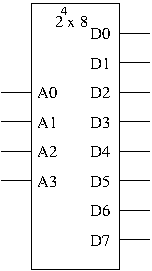
\includegraphics{128BitROM}
  \end{center}
  How many bits does this ROM store?
\end{frame}

This is a 128-bit $2^4$x8 ROM.

\section{ROM Implementations}

\begin{frame}{ROM really isn't memory}
  \begin{block}{Surprising insight}
    Look at the definition of a ROM again.  It is a combinational circuit, so it has no memory (latches or flip-flops).
  \end{block}
  \begin{itemize}
    \item Instead of think of a truth table as a description of a function, let's think of it as an array of data.
    \item The simplest types of ROM are logic gates.
    \item It should not be surprising then that ROM is often implemented using standard combinational logic.
  \end{itemize}
\end{frame}

\begin{frame}{How does it really work?}
  \begin{center}
    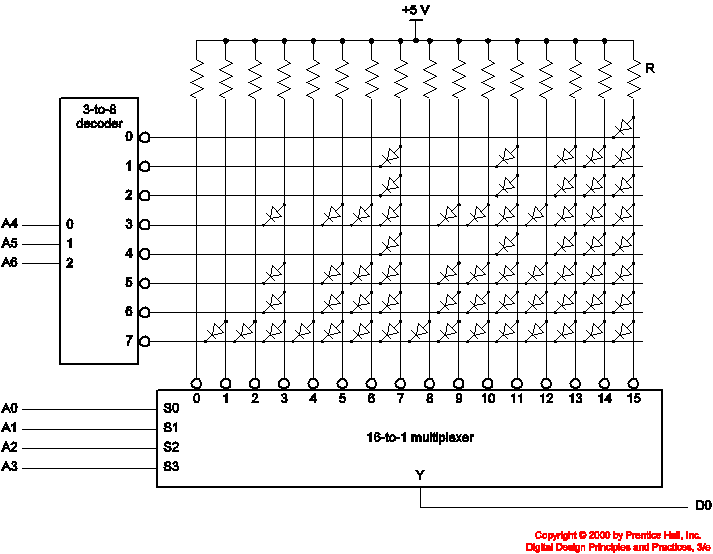
\includegraphics[scale=0.4]{ROMStructure}
  \end{center}
\end{frame}

\section{Types of ROM}

\begin{frame}{Types of ROM}
  ROM is usually categorized based on how it can be programmed.
  \begin{itemize}
    \item Mask ROM
    \item Programmable ROM (PROM)
    \item Erasable programmable ROM (EPROM)
    \item Electronically erasable programmable ROM (EEPROM)
    \item Flash EPROM
  \end{itemize}
\end{frame}

\begin{frame}{Mask ROM}
  \begin{itemize}
    \item This is the oldest type of ROM.
    \item The designer specifies a mask of connections in the ROM array to the manufacturer.
    \item Turn-around time is long, so mistakes can have a tremendous impact.
    \item Used only in high volume applications.
  \end{itemize}
\end{frame}

\begin{frame}{Programmable ROM (PROM)}
  \begin{itemize}
    \item This type of ROM can be modified using a ROM programmer.
    \item All diodes are initially connected, the programmer removes unwanted connections.
    \item Programming is a one-time procedure.
  \end{itemize}
\end{frame}

\begin{frame}{Erasable programmable ROM (EPROM)}
  \begin{itemize}
    \item This type is similar to PROM, but it can be erased using ultraviolet light.
    \item Typically these chips have a window, and sometimes a sticker that covers the window.
    \item A special eraser is used to expose the chip to UV light for a number of minutes.
  \end{itemize}
\end{frame}

\begin{frame}{Electronically erasable programmable ROM (EEPROM)}
  \begin{itemize}
    \item Individual bits may be written electronically.
    \item Only a limited number of writes are possible.
    \item Writing is much slower than reading (usually by at least an order of magnitude).
  \end{itemize}
\end{frame}

\begin{frame}{Flash EEPROM}
  Due to the speed difference between reading and writing EEPROM, flash EEPROM was developed.
  \begin{itemize}
    \item Writes (changing bits to 1) must be done at the block level (typically a large number of bytes).
    \item Changes to bits from 1 to 0 can be done at the bit level.
    \item Flash is subject to memory wear (limited number of writes), but it has been a focus of much recent research.
  \end{itemize}
  Some file systems have special modes of operation to deal with flash memory.
\end{frame}

\section{Flash Memory Application - Data Centers}

\begin{frame}{Flash memory in action}
  The success of Google and services like Amazon's EC3 have made data centers one of the biggest engineering challenges in computing.
  \begin{itemize}
    \item Power consumption is the overwhelming cost for a data center.
    \item Most data centers use off the shelf PC hardware, so reliability is important.
  \end{itemize}
  Although flash memory has had good success in the consumer market (iPods, flash drives, etc.) it may have its largest impact in the data center market.
\end{frame}

\begin{frame}{Budding research}
  A recent research article appeared in CACM that discusses the following applications of flash memory in data centers.
  \begin{itemize}
    \item The impact of flash memory behavior on data centers.
    \item Architectures which extenuate the benefits of flash memory while attempting to mitigate the disadvantages.
  \end{itemize}
\end{frame}

\begin{itemize}
  \item Data center cost (show figure 1)
  \item Flash wear/garbage collection (figure 2b)
  \item Types of flash usage
    \begin{itemize}
      \item Extended memory usage.
      \item Storage accelerator.
      \item Alternative storage device.
    \end{itemize}
  \item Architecture (figure 3)
  \item Read and write regions separate - speeds up garbage collection (figure 4)
  \item Block diagram with variable ECC strength (figure 6)
  \item Results (figures 8 and 10)
\end{itemize}

\end{document}
